\chapter{String Theory and M-Theory}

We begin, as the lecture does, from the particle and only then pass to the string. The reason is not pedagogical caution for its own sake. The whole logic of the chapter is that the string inherits the same basic structure: an action, an exponential weight, and a sum over histories. What changes is that a trajectory becomes a worldsheet, a one-dimensional parameter becomes two coordinates \((\sigma,\tau)\), and the ordinary wave equation gives way, after the familiar Euclidean trick, to a two-dimensional Laplace equation whose conformal invariance is the key to the geometry of string scattering.

\section{From Particle Trajectories to Path Integrals}

For an ordinary particle the first description is classical. In nonrelativistic mechanics we think of the position \(x\) as a function of time \(t\), and for a free particle with unit mass the action is
\begin{equation}
S_{\mathrm{NR}}=\int dt\,\frac12 \dot{x}^{\,2}.
\end{equation}
In the relativistic setting it is more natural to collect the spacetime coordinates into \(X^\mu\) and regard them as functions of a parameter \(\tau\) along the trajectory. In the lecture \(\tau\) is taken to be proper time. The relativistic action is then written in the same spirit,
\begin{equation}
S_{\mathrm{rel}}\sim \int d\tau\,\frac{dX^\mu}{d\tau}\frac{dX_\mu}{d\tau},
\end{equation}
with the understanding that one upper and one lower index are contracted with the spacetime metric.

Classically, in either language, we minimize the action subject to fixed endpoints. The resulting trajectory is the straight worldline of constant velocity. Quantum mechanically, however, the question changes. We are no longer asking which trajectory the particle follows. We ask for the amplitude that a particle prepared at one endpoint is later found at another. This is the path-integral version of the principle of least action:
\begin{equation}
K(1\to 2)=\int \mathcal{D}x\,e^{iS[x]}.
\end{equation}
The relativistic version of this amplitude is the propagator. More complicated processes are obtained by piecing together segments, integrating over joining points, and finally summing over diagrams.

The point to retain is the change of question. The action is still central, but it is no longer minimized directly. It is exponentiated and then summed over histories.

\section{The Physicist's Cheat: Turning Time Sideways}

The lecture pauses here to raise the obvious objection. If the integrand is \(e^{iS}\), then every history contributes with unit magnitude. The difference between tame and wild histories is only in phase. That is enough for formal interference, but it is not enough to make the integral converge in any naive sense.

\subsection{Question \& Answer}

\paragraph{Question.} Why does the oscillatory path integral need help at all?

\paragraph{Answer.} Because wildly varying paths are not numerically suppressed. A path that shoots off to a great distance and returns, or one that wiggles violently, contributes an integrand of magnitude one just as a nearly classical path does. The classical path can dominate only after delicate cancellations, and that is not a mathematically friendly starting point.

The trick is the standard one. Reparameterize the trajectory by
\begin{equation}
\tau=\alpha s.
\end{equation}
Then
\begin{equation}
d\tau=\alpha\,ds,
\qquad
\frac{dX}{d\tau}=\frac{1}{\alpha}\frac{dX}{ds},
\end{equation}
so the quadratic action becomes
\begin{equation}
\int d\tau\,\left(\frac{dX}{d\tau}\right)^2
=
\frac{1}{\alpha}\int ds\,\left(\frac{dX}{ds}\right)^2.
\end{equation}
Choosing \(\alpha=-i\) turns the phase into a decaying exponential. Up to the same unimportant overall normalization conventions used in the lecture,
\begin{equation}
e^{iS}
\longrightarrow
\exp\!\left[-\frac12\int ds\,\left(\frac{dX}{ds}\right)^2\right].
\end{equation}
This is the convergent Euclidean form. Histories with large derivatives now carry a large positive action and are exponentially suppressed.

The lecture is explicit that this move is a cheat before it is a theorem. One calculates the Euclidean object first and then analytically continues back to the desired complex values of the parameters. For present purposes that is the operative definition of how path integrals are actually used.

\section{From Worldlines to Worldsheets}

Now we lift the whole discussion to strings. A particle is replaced by an extended object, and its history is no longer a worldline but a two-dimensional surface. For an open string that surface is ribbon-like; for a closed string it is tube-like. In either case we use two internal coordinates \((\sigma,\tau)\) on the worldsheet and describe the embedding into spacetime by
\begin{equation}
X^\mu=X^\mu(\sigma,\tau).
\end{equation}

The action is the immediate two-dimensional generalization of the particle action. The board evidence secures the derivative structure, though not the full normalization. We therefore write it in the canonical schematic form
\begin{equation}
S_{\text{ws}}
\propto
\int d\tau\,d\sigma
\left[
\left(\partial_\tau X^\mu\right)^2
-
\left(\partial_\sigma X^\mu\right)^2
\right].
\end{equation}
The first term is the kinetic term along the worldsheet time direction; the second plays the role of potential energy and carries the opposite sign.

\begin{figure}
\centering

\includegraphics[width=0.62\textwidth]{lecture_07_figure_02.png}
\caption{Blackboard evidence for the worldsheet action density: a \(\tau\)-derivative term opposed by a \(\sigma\)-derivative term. The full coefficient and measure are not fixed by the frame alone.}
\end{figure}

Quantum mechanically we exponentiate this action and integrate over all worldsheets interpolating between the prescribed initial and final string configurations:
\begin{equation}
\mathcal{A}
=
\int \mathcal{D}X\,e^{iS_{\text{ws}}[X]}.
\end{equation}
If the initial state contains two strings and the final state contains three, we sum over all surfaces with that boundary data. If we include holes and more general topologies, we recover the analog of summing over all Feynman diagrams.

The lecture also insists on one important bridge back to ordinary particle physics: at sufficiently low energies, compared with the string scale, these amplitudes reproduce ordinary Feynman-diagram physics. That point is not derived here, but it is used to keep the whole construction anchored to familiar quantum theory.

\begin{remark}
Susskind briefly notes a more geometrically motivated form of the action: proper length for a particle and worldsheet area for a string. In modern language that is the Nambu--Goto point of view. He also mentions the Polyakov and Liouville names as part of the history of the subject, but those formalisms are not used in the present lecture.
\end{remark}

\section{Euclidean Equation of Motion and the Laplace Form}

The worldsheet path integral suffers from the same disease as the particle path integral: wildly fluctuating surfaces are not suppressed in the oscillatory form. So we make the same Euclidean move on the worldsheet time variable. The lecture works through the signs live on the board and corrects itself in real time; for the notes it is better to keep one consistent outcome in view. After the Wick rotation, both derivative terms appear with the same sign inside the Euclidean action, so that rough or far-reaching surfaces are exponentially damped.

Instead of studying the action directly, Susskind then switches to the equation of motion. This is not a change of subject. It is a more transparent way to see what coordinate changes preserve the structure of the theory.

\subsection{Question \& Answer}

\paragraph{Question.} Why does the board now display a plus-sign equation rather than the ordinary Lorentzian wave equation?

\paragraph{Answer.} Because the lecture has already turned \(\tau\) into Euclidean time. Before that move the string equation has the wave-equation form
\begin{equation}
\partial_\tau^2 X-\partial_\sigma^2 X=0.
\end{equation}
After the Euclidean continuation the sign changes, and the equation becomes
\begin{equation}
\partial_\tau^2 X+\partial_\sigma^2 X=0.
\end{equation}
That is the two-dimensional Laplace equation on the worldsheet.

\begin{figure}
\centering

\includegraphics[width=0.64\textwidth]{lecture_07_figure_03.png}
\caption{The Euclideanized worldsheet equation on the board, together with the first discrete geometric picture.}
\end{figure}

We may think of \(X\) here as one component of \(X^\mu\). Mathematically it behaves just like an ordinary scalar field obeying the Laplace equation in two variables, except that the two variables are now the worldsheet coordinates \(\sigma\) and \(\tau\).

\begin{figure}
\centering
\begin{tikzpicture}[scale=1]
\draw (-4,0) -- (4,0);
\foreach \x in {-3.7,-3.3,-2.9,-2.5,-2.1,-1.7,-1.3,-0.9,-0.5,-0.1,0.3,0.7,1.1,1.5,1.9,2.3,2.7,3.1,3.5}
  \draw (\x,-0.08) -- (\x,0.08);
\end{tikzpicture}
\caption{A clean redraw of the discretized line that begins the geometric interpretation of the second derivative.}
\end{figure}

\section{Discrete Derivatives and the Average-Value Property}

The lecture now slows down deliberately. Rather than invoke the Laplace equation as an abstract PDE, it asks what the second derivative means geometrically.

On a discrete line with neighboring points \(1,2,3\), a first derivative is represented by a first difference. Ignoring the common factor of the lattice spacing \(\epsilon\), the second derivative is the difference of first differences:
\begin{align}
\partial^2 X
&\leadsto
\bigl[X(3)-X(2)\bigr]-\bigl[X(2)-X(1)\bigr] \\
&=
X(3)+X(1)-2X(2).
\end{align}

\begin{figure}
\centering

\includegraphics[width=0.72\textwidth]{lecture_07_figure_04.png}
\caption{The finite-difference development on the blackboard: the same Laplace-form equation, a numbered discrete line, a lattice patch, and the simplified second-difference formula.}
\end{figure}

\begin{figure}
\centering
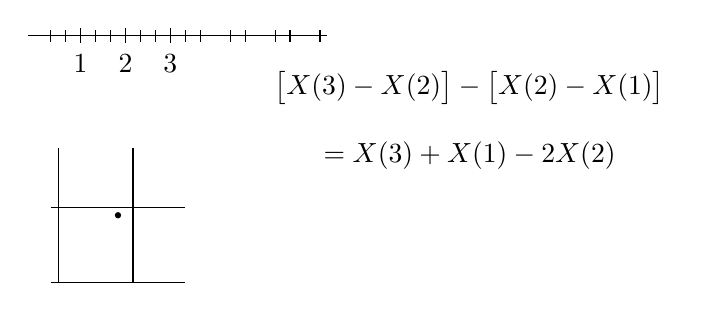
\begin{tikzpicture}[scale=0.95]
\draw (-4.4,2.3) -- (-0.4,2.3);
\foreach \x/\lab in {-3.7/1,-3.1/2,-2.5/3}
{
  \draw (\x,2.2) -- (\x,2.4);
  \node[below] at (\x,2.18) {\(\lab\)};
}
\foreach \x in {-4.1,-3.9,-3.5,-3.3,-2.9,-2.7,-2.3,-2.1,-1.7,-1.5,-1.1,-0.9,-0.5}
  \draw (\x,2.22) -- (\x,2.38);

\draw (-4.1,0.8) grid (-2.3,-1.0);
\fill (-3.2,-0.1) circle (1.2pt);

\node at (1.5,1.6) {\(\bigl[X(3)-X(2)\bigr]-\bigl[X(2)-X(1)\bigr]\)};
\node at (1.5,0.7) {\(=X(3)+X(1)-2X(2)\)};
\end{tikzpicture}
\caption{A clean redraw of the one-dimensional finite-difference formula and the lattice picture that leads into the two-dimensional Laplacian.}
\end{figure}

Now pass from the line to a discrete \((\sigma,\tau)\)-plane. Let the four nearest neighbors of a central point \(5\) be labeled \(1,2,3,4\). Then the two second derivatives are represented by
\begin{equation}
\partial_\tau^2 X \leadsto X(1)+X(3)-2X(5),
\qquad
\partial_\sigma^2 X \leadsto X(2)+X(4)-2X(5).
\end{equation}
The Laplace equation therefore becomes
\begin{align}
0
&=
\bigl[X(1)+X(3)-2X(5)\bigr]
+
\bigl[X(2)+X(4)-2X(5)\bigr] \\
&=
X(1)+X(2)+X(3)+X(4)-4X(5).
\end{align}
Equivalently,
\begin{equation}
X(5)=\frac14\bigl[X(1)+X(2)+X(3)+X(4)\bigr].
\end{equation}

\subsection{Question \& Answer}

\paragraph{Question.} What does the Laplace equation mean geometrically at a point?

\paragraph{Answer.} It says that the value at the center of an infinitesimal square is the average of the values at the corners. This is the local geometric content of the Laplace equation. The square may be rotated; the statement is invariant under rotations of the \((\sigma,\tau)\)-plane.

This is the crucial step in the lecture. The Laplace equation ceases to be merely algebraic and becomes a geometric averaging principle.

\section{Conformal Invariance of the Worldsheet}

Once the Laplace equation has been rewritten as an average-value property on infinitesimal squares, the right invariance group is almost forced on us. We must ask for coordinate transformations of the worldsheet that preserve the class of infinitesimal squares. Those are precisely the transformations under which the average-value statement remains true.

Susskind first phrases the answer in terms of squares and then in terms of angles. A transformation that preserves all angles takes infinitesimal squares to infinitesimal squares, though it may rescale them by a position-dependent factor. Thus the relevant invariance is conformal invariance.

In the lecture this point is elaborated with a useful warning. Conformal maps preserve local shape, not global size. A tiny square can map to a larger or smaller tiny square. A finite region with boundary may be carried to a very different-looking finite region, because corners need not map to corners. The preservation is local and infinitesimal, not rigid.

There is also a brief aside that coordinate transformations generated by analytic functions of a complex variable are angle-preserving. That remark is not pushed technically here, but it prepares the return to the scattering geometry.

\section{From the Band-Aid to the Disc and Back to Duality}

The lecture now comes back to the string-splitting worldsheet from the previous meeting: a slit ribbon, or what Susskind jokingly calls an infinite sports band-aid. Two strings join into one, propagate for a while, and split again. The original picture has a visible time interval between the joining and the splitting, and in the end one integrates over that interval. That integral gives the Euler beta function, or Veneziano amplitude.

The new point is that after Euclideanization the same problem can be conformally mapped to a disc. The fields \(X^\mu(\sigma,\tau)\) may now be regarded as living on the disc rather than on the slit strip, and the form of the Laplace equation is unchanged.

\subsection{Question \& Answer}

\paragraph{Question.} Why do four boundary insertion points leave only one real parameter?

\paragraph{Answer.} Because conformal transformations on the disc still allow us to move boundary points around. Once we use that freedom to impose a convenient symmetric placement, only one genuine modulus remains. In the lecture this surviving modulus is the disc-language counterpart of the original joining--splitting time interval on the slit worldsheet.

There are four distinguished boundary points on the disc, carrying the data of the external string states. The lecture does not yet develop the full formalism, but it indicates the modern answer: one inserts vertex operators at those special points.

A convenient symmetric representative is a disc with four boundary points arranged with left-right and up-down symmetry. The remaining one-parameter freedom then slides the points through a family of configurations. One extreme corresponds to a long-lived intermediate string in the direct channel; the other to the crossed-channel picture.

\begin{figure}
\centering
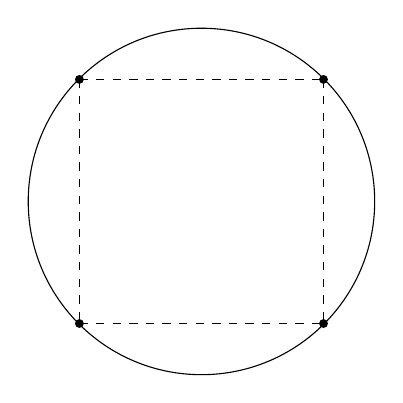
\begin{tikzpicture}[scale=1.0]
\draw (0,0) circle (2.2);
\fill (-1.55,1.55) circle (1.6pt);
\fill (1.55,1.55) circle (1.6pt);
\fill (-1.55,-1.55) circle (1.6pt);
\fill (1.55,-1.55) circle (1.6pt);
\draw[dashed] (-1.55,1.55) -- (1.55,1.55);
\draw[dashed] (-1.55,-1.55) -- (1.55,-1.55);
\draw[dashed] (-1.55,1.55) -- (-1.55,-1.55);
\draw[dashed] (1.55,1.55) -- (1.55,-1.55);
\end{tikzpicture}
\caption{A schematic disc picture with four special boundary points. The lecture's stable content is that, after quotienting by conformal symmetry, only one real parameter remains.}
\end{figure}

The board sketches at the end of the lecture emphasize the symmetry between the two extreme channels.

\begin{figure}
\centering

\includegraphics[width=0.56\textwidth]{lecture_07_figure_06.png}
\caption{The paired end-of-lecture sketches that display the symmetry between the two extreme channel pictures.}
\end{figure}

\begin{figure}
\centering
\begin{tikzpicture}[scale=0.95]
\draw (-3,1.8) -- (-1.0,0.3);
\draw (-3,4.6) -- (-1.0,3.1);
\draw (3,1.8) -- (1.0,0.3);
\draw (3,4.6) -- (1.0,3.1);
\draw (-1.0,3.1) -- (-0.5,3.35);
\draw (-0.5,3.35) -- (0.0,3.1);
\draw (0.0,3.1) -- (0.5,3.35);
\draw (0.5,3.35) -- (1.0,3.1);

\draw (-3,-4.6) -- (-1.0,-3.1);
\draw (-3,-1.8) -- (-1.0,-0.3);
\draw (3,-4.6) -- (1.0,-3.1);
\draw (3,-1.8) -- (1.0,-0.3);
\draw (0.0,-3.1) -- (0.25,-2.55);
\draw (0.25,-2.55) -- (0.0,-2.0);
\draw (0.0,-2.0) -- (0.25,-1.45);
\draw (0.25,-1.45) -- (0.0,-0.9);
\draw (-1.0,-3.1) -- (0.0,-3.1);
\draw (-1.0,-0.3) -- (0.0,-0.9);
\draw (1.0,-3.1) -- (0.25,-3.1);
\draw (1.0,-0.3) -- (0.25,-0.9);
\end{tikzpicture}
\caption{A clean redraw of the two symmetric interaction sketches. The point is geometric symmetry, not detailed labeling.}
\end{figure}

The stable kinematic identifications are the Mandelstam variables
\begin{equation}
s=(k_1+k_2)^2,
\qquad
t=(k_1+k_3)^2,
\end{equation}
with all momenta taken incoming. The lecture's final claim is then that the same integral accounts for both channels. What looked miraculous in the old band-aid picture becomes natural in the conformally mapped one: the amplitude is symmetric under the interchange of the two channel descriptions,
\begin{equation}
\mathcal{A}(s,t)=\mathcal{A}(t,s).
\end{equation}
This is the original channel duality.

\section{Summary}

The lecture begins with the ordinary particle in order to teach us how to read string theory. First comes the action, then the quantum amplitude, then the Wick rotation that makes the path integral manageable. Only after that does the string worldsheet appear.

Once the string action has been Euclideanized, its equation of motion becomes the Laplace equation. The Laplace equation, interpreted geometrically, tells us that the value at the center of an infinitesimal square is the average of the values at the corners. That local statement singles out conformal transformations as the natural coordinate freedom on the worldsheet.

Finally, conformal invariance reshapes the awkward slit-strip scattering surface into the disc. In that picture the four-point amplitude depends on a single modulus, and the two apparently different channel limits are seen to be two ends of the same integral. That is the mathematical core of the lecture, and it is also the first glimpse of the duality that made string theory so compelling in the first place.